\chapter{EVENT LOCALIZATION}
 \label{chap:eventLo}
\section{Introduction}
Video event localization has been extensively studied with an objective to locate the action of interest but locating an event in video, typically suffers from an enormous combinatorial complexity.  Generally output of such a task encompasses action of interest by a sub-volume.  The task can be considered to be difficult than event recognition because localized actions are present only on fraction of the frames in a video.  Some of the common strategies that are tried on this kind of problems are efficient sub-window search ~\citep{subwindowsearch},"selective search" strategy ~\citep{selectivesearch}  and ~\cite{tubelet}, but these either perform exhaustive search or perform iterative merging of the supervoxels. 

\par This chapter has been sectioned into four parts.  In Section \ref{sec:bst} approaches for capturing the pixels that are in motion is discussed.  Then techniques for extracting the salient regions in a given frame is explained in Section \ref{sec:sal}.  The craft for fusing the above two techniques is examined in Section \ref{sec:ts} and in Section \ref{sec:trac} way for obtaining spatio-temporal volume is elaborated.

\section{Background Subtraction Techniques} 
 \label{sec:bst}
\par One simple approach ~\citep{Basharat08} for the event localization was to understand the motion relativity and the position of pixel changes, this is based on inspiration that components corresponding to an event show a similar flow of pixels.  This approach works significantly well in surveillance data but fails for human event detection.  It was later realized that, by eliminating the background(static parts) of the visual frame,  possible event locations can be retained.  Several background subtraction techniques are available in \cite{Piccardi04}, among these some apply on static image while others on dynamic video.  In case of our application we can blend both these approaches to generate more reliable event detectors.

\subsection{Frame Differencing (FD)}
A very common approach for performing the moving object segmentation is using frame differencing but this approach is very sensitive to small changes and yields lots of noise when a camera is in motion.  A simpler way to implement this technique is to compute the absolute difference of gray scale/intensity values across consecutive frames. Consider $P(p_x,p_y,t)$, intensity of pixel $(p_x,p_y)$ at frame t, then pixel $(p_x,p_y)$ is considered foreground when absolute difference is above a threshold,$$\vert P(p_x,p_y,t+1) - P(p_x,p_y,t)t\vert > T$$.
\par The robustness of this method depends on speed of foreground elements.  Faster movements may require higher thresholds to reduce the noise.   An alternate approach is to replace difference of a single previous frame  by an average of multiple previous frames, still results are noisy and not reliable.

\subsection{Mixture of Gaussian (MOG)}
MOG is one of the well known method of extracting foreground information.  As per \cite{kaew}, background pixels were modelled by a mixture of N Gaussian distributions.  The mixture weights represent the proportions that these colors are retained in the frame while the colors that are static and staying longer are probably background.  At any instance $i$ a particular pixel $(p_x,p_y)$ has color space represented as $V(p_{x},p_{y},i)$,  history of the pixels are given by 
$$X_{1},..,X_{t} = {V(p_{x},p_{y},i)~:~1\le i \le t }$$
The history is modelled by mixture of N Gaussian mixtures,
$$P(X_{t})=\Sigma_{i}^{N}w_{i,t}\eta(X_{t}|\mu_{i,t},\Sigma_{i,t})$$
\par $w_{i,t}$, $\mu_{i,t}$, $\Sigma_{i,t}$ are weight, mean and covariance of the $i^{th}$ Gaussian in the mixture at time $t$ respectively and where $\eta$ is the Gaussian density function.  The general principle behind this approach is that when a foreground object blocks the background object, the color distributions will begin to change resulting in either the creation of a new distribution or the increase in the variance of an existing distribution.  The foreground object that is in motion is expected to have a larger variance compared to background pixel until the foreground object halts.


\subsection{Eigen subtraction (ES)}
Eigen based background subtraction was considered as an elegant method compared to the methods discussed above.  A sample of N images of the videos are obtained, mean background image $\nu_b$ is computed and all images are mean normalized  $X$.  Principal component analysis on the mean normalized images is performed, with an idea that a high-dimensional images are often described by correlated variables and only a few meaningful dimensions account for most of the information.  But performing PCA for large images is not straightforward, consider 100 images of dimension 100x100 pixels, then the dimension of generated covariance matrix would be 10000x10000, i.e roughly 0.8 GB (considering 64 bit float values). Solving this is not feasible, hence a trick from linear algebra that for a MXN matrix with $M>N$, can at most have N-1 non-zero eigenvalues ~\cite{Duda01} can be used. Eigenvalue decomposition of $X^TX$ is carried out:
$$X^TX\nu_i=\lambda_i\nu_i$$
$$XX^T(X\nu_i)=\lambda_i(X\nu_i)$$
The orthonormal eigenvector of $XX^T$ is found out by normalizing $X\nu_i$ to unit length.  Once eigenvectors of $XX^T$  are computed, projection of the current frame $F$ on the eigenvectors with top eigenvalues are determined, and the reconstructed frame $F'$ is obtained by using the projection coefficients and the eigenvectors.  The difference $F-F'$ would correspond to the mask on the moving object.

\begin{figure}[htpb]
   \begin{center}
	    \includegraphics[width=0.75\textwidth]{snaps/bgsub/results.eps}     
     \caption {Background subtraction techniques on multiple video classes}
   \label{fig:bgsub}
   \end{center}
 \end{figure}
\par Results of foreground mask obtained using FD, ES and MOG are shown in Figure \ref{fig:bgsub}. Even though MOG is most preferred, but found it provide sparse and not a clear boundary in most of the sample videos.  In "dance" video, the FD yields extraneous pixels due to camera movement in between two dancers, which are not evident in ES and MOG.  Also FD produces spurious pixels for the "pommello" video, because of the sharp background.  All methods fail in case of grainy videos, hence background subtraction alone can not be suffice for the event localization.

\section{Saliency Detection}
\label{sec:sal}
Visual saliency is a unique perceptual aspect that makes some items in the world stand out from their neighbours and grab attention on it immediately.  As we had discussed earlier about the different techniques to extract the eminent pixels which are in motion, sometimes pixels which are stationary and quite distinct might also play a important role in the the activity recognition.  Visual saliency are considered in attention modelling.  Most of saliency estimations techniques follow the following five steps which can be visualized in Figure \ref{fig:salap},
\begin{itemize}
\item{\textbf{Step 1: Color equalization:} This is performed by removing the tail in the color histogram.  It helps improving the contrast in the image.  In the implementation color equalization is done on each channel separately so that all channels can be provided to the segmentation algorithm.}

\item{ \textbf{Step 2: SLIC-based segmentation:}  It is a simple linear iterative clustering that clusters pixels in the combined five-dimensional color and image plane space to efficiently generate compact, nearly uniform super-pixels.  Any slic based clustering algorithm takes two parameters number of super-pixels and compactness of each super-pixel.  According to \cite{slic}, slic is fastest and most memory efficient compared to  other segmentation technique like graph-cut, quick shift segmentation techniques.  Segmentation reduces the number of computation in the subsequent stages.}

\item{ \textbf{Step 3: Extract segment properties:} Extracting features of the region that are used in computing the saliency of each region.  Some features that are considered in the implementation are color based features (LAB,RGB) and texture based features (GLCM,Texture Flow).}

\item{\textbf{Step 4: Compute~saliency:} Saliency estimation techniques can be broadly categorized into bottom-up, top-down and information maximization based on algorithmic computation. Earliest saliency based attention modelling was proposed by \cite{itti}.  It was inspired by the behaviour and the neuronal architecture of the early primate visual system.}

\item{\textbf{Step 5: Saliency cut:} Saliency maps are generally thresholded to obtain the salient mask.  In the implementation, grab-cut\citep{grab-cut} performs segmentation by modelling foreground and background based on saliency estimation to obtain the mask where higher saliency  contemplate foreground while lower saliency estimate correspond to background.  Once saliency mask are obtained few morphological operation are applied to remove the salt and pepper noise.}
\end{itemize}

\begin{figure}[htpb]
   \begin{center}
	    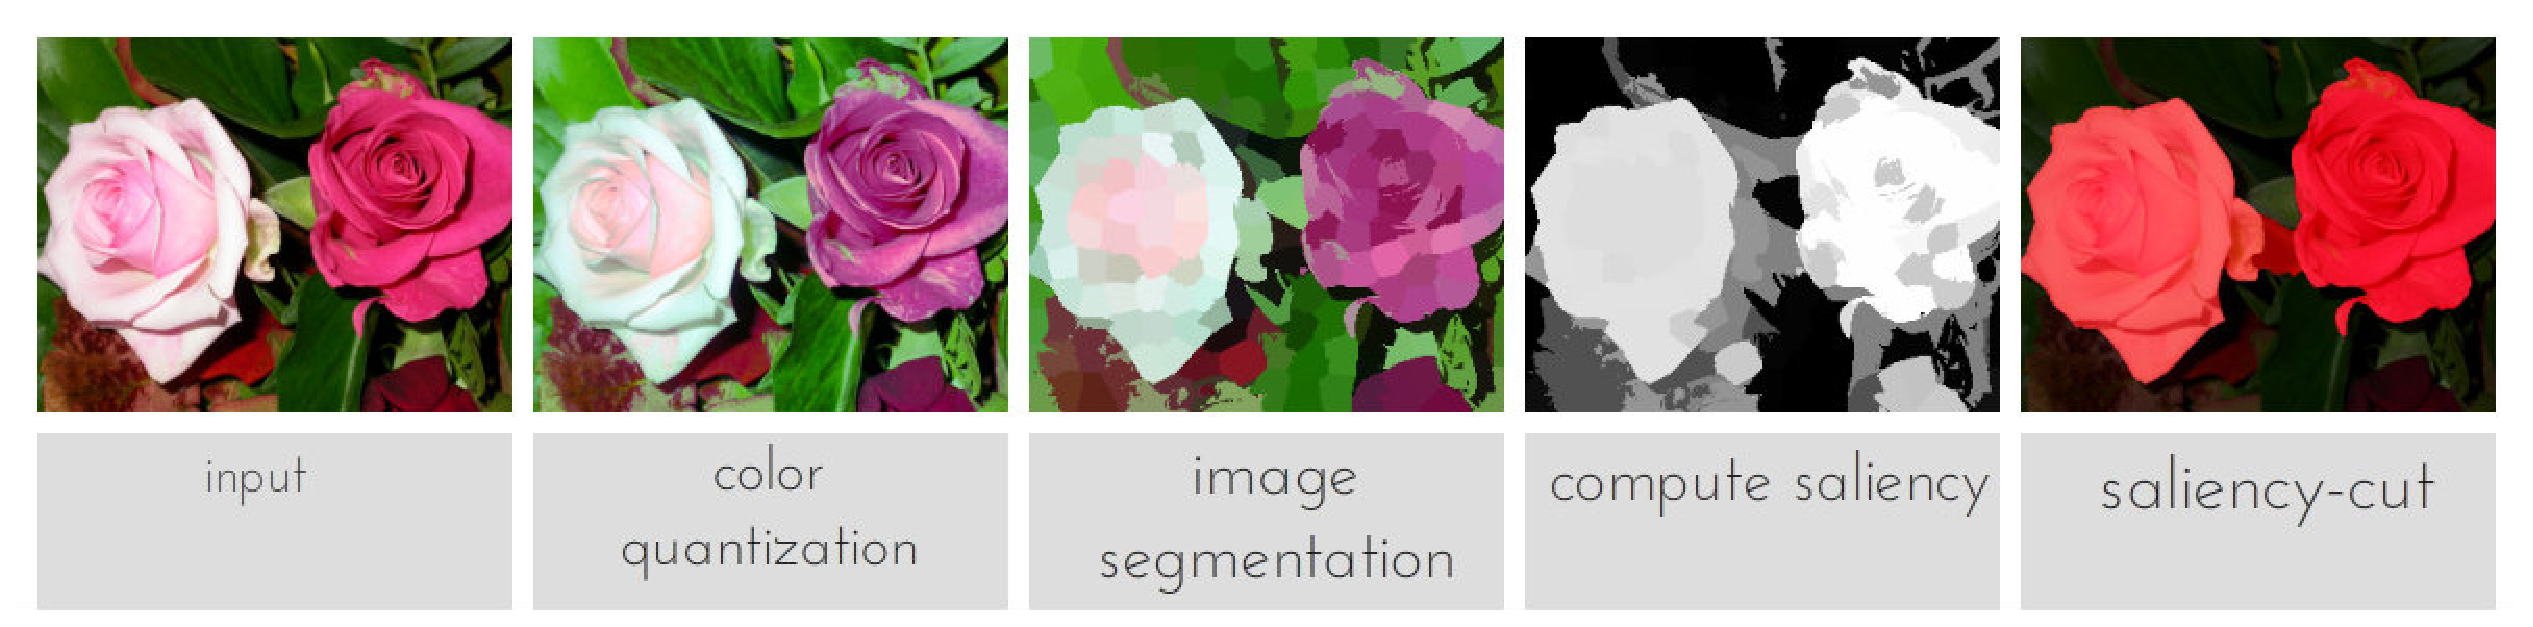
\includegraphics[width=0.95\textwidth]{snaps/sal/saliency.eps}     
     \caption {A general approach for saliency estimation}
   \label{fig:salap}
   \end{center}
 \end{figure}

\par Different saliency estimation techniques that were studied are discussed below.  All these techniques can be considered either at region level or pixel level, based on whether the segmentation of the image is considered or not.

\subsection{Hierarchical Color Based (HCB)}
HCB is a top-down approach for computing saliency where saliency map of improbable pixels/regions are set to zero at every iteration.  Saliency of pixel/region $I_{x}$ is computed as follows,
$$ Iavg_{x} = \Sigma_{y} I_{y}~\exp^{-\frac{\parallel~p_{x} - p_{y}~\parallel}{w}}  $$
$$ saliency(I_{x}) =~\parallel I_{x} - Iavg_{x} \parallel $$
where $p_{x}$ is the position of the pixel $I_{x}$.  At each iteration, the $w$ is decreased implying closer neighbourhood.  After each iteration pixels/regions with $ saliency(I_{x})$ lesser than $0.1$ after normalization are eliminated.  In this manner, the foreground pixels/regions are obtained by discarding the background pixels/regions.  The primary focus is to measure the variation from the average pixel intensity.

\subsection{Context Aware Based (CAB)}
In CAB, saliency estimate are averaged out at a different context windows.  The expressions for the estimation of saliency is given below,
$$ AllPairDistance(I_{x},I_{y},k) = \exp^{-\frac{\parallel~p_x - p_y~\parallel}{dw_k}}~\exp^{-\frac{\parallel~I_{x} - I_{y}~\parallel}{cw}}$$
$$ NormDistance(I_{y},k) = \Sigma_{x} AllPairDistance(I_{x},I_{y},k)$$
$$ saliency(I_{x}) = 1- \Sigma^{K}_{k=1}~dw_{k}~\Sigma_{y}~\frac{AllPairDistance(I_{x},I_{y},k)}{NormDistance(I_{y},k)}$$
where $cw$ and $K$ are color weight and number of context windows respectively.  Saliency measures the similarity with its neighbourhood weighted on proximity of the pixels/regions. $AllPairDistance(I_{x},I_{y},k)$ is disparity measure across pairs of pixels/regions $(I_{x},I_{y})$ for different values of $dw_{k}$ while $NormDistance(I_{y},k)$ correspond to the normalizing factor. This technique perform fairly well in discriminating salient objects which are not in same scale.

\subsection{Spectral Distribution Based (SDB)} 
SDB is based on the intuition that pixels with small color distribution variances have high saliency values.  The extent of color distribution is measured from the spatial variance of all colors in the image.  \cite{spectralSal} proposed a technique to compute color spatial variances using Gaussian Mixture Models (GMMs).  All pixels/regions in the image are represented by GMMs using expectation maximization (EM) algorithm, where $w_{c}$, $\mu_{c}$ $\Sigma_{c}$ is the weight, the mean color, and the covariance matrix of the $c^{th}$ mixture. Each pixel/region is assigned to a mixture with the probability:
$$p(c | I_{x}) = \frac{w_{c}\eta(I_{x}| \mu_{c},\Sigma_{c})}{\Sigma_{c}w_{c}\eta(I_{x}| \mu_{c},\Sigma_{c}} $$
Suppose $x_{h}$ is the x coordinate (horizontal coordinate) of the pixel x. The spatial variance for x-dimension of color component c is computed as:
$$\sigma_{h}^{2}(c) = \frac{1}{|P|_{c}}\Sigma_{x}	p(c | I_{x}) \parallel x_{h} -M_{h}(c) \parallel^{2}$$
where $M_{h}(c) = \frac{1}{|P|_{c}}\Sigma_{x}p(c|I_{x})~x_h$ , and $|P|_{c} = \Sigma_{x}p(c | I_{x})$ is a normalization factor.  The vertical variance $\sigma_{v}^{2}(c)$ is defined similarly.  The spatial variance of a component c is combined as: $\sigma^{2}(c) = \sigma_{h}^{2}(c) + \sigma_{c}^{2}(c)$ which is then normalized.
The saliency $saliency(I_{x})$ of a specific pixel $I_{x}$ regarding to color spatial distribution is defined as the weighted sum:
$$saliency(I_{x}) = \Sigma_{x}p(c | I_{x})(1-\sigma^{2}(x))$$
This method yields very good results for many examples but the configurations requires tweaks for better results.

\subsection{Regional Contrast (RC)}
RC computes saliency of an image region by measuring contrast with respect to the entire image. Several approaches  \citep{globContrast}, {patchRarities}, \citep{salFilters} for computing saliency based on global contrast are known in the literature while in this work, different techniques are fused and presented.  It considers two contrast measures:
\subsubsection{Uniqueness}
Element uniqueness is contemplated with the assumption that image regions, which stand out from other regions in certain aspects, catch our attention and hence must be labelled as more salient.  Element uniqueness for segment $I_{x}$, given its position $p_{I_{x}}$ compared to all other $I_{y}$ is defined as follows,
$$uniqueness(I_{x}) = \Sigma_{y} \parallel~I_{x} -I_{y}~\parallel~\exp^{-\frac{\parallel~p_{x} - p_{y}~\parallel}{dw}}$$
where $dw$ controls the proximity of the neighbourhood, higher value correspond to wider neighbourhood.
\subsubsection{Distribution}
In general, colors belonging to the background will be distributed over the entire image exhibiting a high spatial variance, whereas foreground objects are generally more compact.  Element distribution measure for a segment $I_{x}$ using the spatial variance of its color as follows,
$$distribution(I_{x}) = \Sigma_{y} \parallel~p_{y} -\mu_{x}~\parallel~\exp^{-\frac{\parallel~I_{x} - I_{y}~\parallel}{cw}}$$ 
where $\mu_{x} = \Sigma_{y}~p_{y}~exp^{-\frac{\parallel~I_{x} - I_{y}~\parallel}{cw}}$, measures weighted mean position of the color of $I_{x}$ component.  Low variance indicates a spatially compact object hence they are considered more salient than spatially widely distributed elements.

\par The two above contrast measures defined at element level can be consolidated by given expression,
$$saliency(I_{x}) = uniqueness(I_{x}) \exp^{-k~distribution(I_{x})}$$
where $k$ controls the emphasis on distribution while both the contrast measure are normalized. It is observed that the uniqueness performs well in case of single object saliency while for multiple object saliency, uniqueness together with distribution yields better result.  Saliency mask obtained using HCB, CAB, SDB and RC for some standard weizmann segmentation dataset images are shown in Figure \ref{fig:sal}. 

\begin{figure}[htpb]
   \begin{center}
	    \includegraphics[width=0.75\textwidth]{snaps/sal/saliencyall.eps}     
     \caption {Saliency mask obtained using multiple techniques}
     \medskip \small 
     Following observation are quite evident from the results, 1. HCB is very sensitive to the weights provided. 2. CAB are generally good but yields lot of false positives. 3. SDB is quite random as it depends on the random seed used in GMM. 4. RC is very robust for most of the example but certainly depends on the weights.
   \label{fig:sal}
   \end{center}
 \end{figure}

 \section{Temporal Smoothening}
  \label{sec:ts}
Smoothening of the event mask obtained at frame level is essential because of occlusion and illumination variations.  A common approach which was followed for the smoothening of frame was by blending the background subtraction measure and the saliency measure to obtain a visual attention score. Higher visual attention score ($\geqslant0.8$) were considered \textsc{True Foreground} while lower visual attention score ($\leqslant0.2$)  were considered \textsc{True Background}.  Then models are built for prediction of other regions/pixels.  Three approaches for smoothening of visual attention measure are described below and in all approaches context before and after the frame is considered.

\subsection{Eigen Based}
Eigen Based method is based on projecting the pixels along the direction of maximum variance for foreground and background.  Any pixel is assigned foreground if the projection along the direction of maximum variance is large along foreground compared to background.  The direction of maximum variance are computed by gathering features (pixel level features like color, texture, gradient and position) of foreground/background pixels in the context and perform the principal component analysis (PCA).  But this approach of smoothening, did not yield good localization.

\subsection{Semi-supervised}
Semi-supervised learning are techniques where in the training data some of the samples are not labelled, this appropriately fits the smoothening task.  In such techniques, the unlabelled data are made use for capturing the manifold of the underlying data distribution thus generalize better for new examples. 
\par In this work, label propagation \citep{labprop}, a graph based semi supervised learning was materialized for polishing the mask.  This technique was computationally intensive as we required to build model using all pixels in the frame for given context.  There was no adaptation mechanism which was available, for a faster convergence of learning algorithm.

\subsection{Gaussian Mixture Based}
Gaussian mixture model was  most successful experiment among the techniques considered.  In this approach, two Gaussian mixture model were built using true foreground and background examples. Each and every pixels are assigned to either foreground or background based on the likelihood scores of foreground and background model.  One of the biggest advantage of this approach is its support to adapt, i.e models of previous frames can be fine-tuned for the current frames which helps training individual context models quickly.

\par Because of the swiftness and the robustness the Gaussian mixture models was examined for all the experiments.  Few post processing operation were carried over the predicted mask like median smoothing, region filling were performed to remove the salt and pepper noises and spurious regions that are small.  Figure \ref{fig:smoothen} shows smoothed mask obtained from from the visual attention score.  It shows how the model captures interesting regions even if their visual attention scores are not so eminent in that frame.
\begin{figure}[!htpb]
   \begin{center}
	    \includegraphics[width=0.75\textwidth]{snaps/smooth/smoothening.eps}     
     \caption {Gaussian mixture based smoothening}
 	\medskip 
 	\small Odd rows depict the visual attention score, with red and green representing true foreground and background respectively.  Even rows illustrate the smoothed mask obtained from the visual attention score using the Gaussian mixture model. 
   \label{fig:smoothen}
   \end{center}
 \end{figure}
 
\section{Tracking}
 \label{sec:trac}
Tracking focuses on drawing a bounding box around a region of interest and tracking of them in a train of frames.  After detecting interesting regions and post-processing operations, the filtered masks are grouped into connected regions (blobs) and labelled by using a connected component labelling algorithm.  The bounding boxes of these blobs correspond to a object/subject are computed by a novel approach.  It ensures mask to be present even if there are any uneventful (no mask) or extremely eventful (too many mask) frame.   This task is accomplished by building two GMM models, one to characterize the location of the event (like x-y coordinates and size) and other to characterize region color properties (like color histogram).  The GMM model built with context of 4-8 frame context gives the location and size of localized region in the frame. 
Back projection \citep{backProj} of region of interest (obtained from mean of GMM model) on the given frame is measured that determines the probability of a pixel belong to the object.  The back-projected image  will have region of interest in white while black for others.  A fine-tuning of the result is attained using the mean shift algorithm.  The intuition behind mean-shift algorithm is simple, the tracking window is shifted until it reaches the area of maximum pixel density.  When the object moves, obviously the movement is reflected in histogram of back-projected image. 
\par In this manner, tracking an event without the knowledge of location of interest is made possible.  The bounding box obtained are of different size, so all windows are extended to the shape largest enclosing one.  All these train of  windows form the spatio-temporal volume (STV). Figure \ref{fig:tracking} depicts STV for multiple events : horse riding, javelin, horse racing and bench press videos.
\begin{figure}[htpb]
   \begin{center}
	    \includegraphics[width=0.75\textwidth]{snaps/track/tracking.eps}     
     \caption {Event tracking after obtaining the smoothened mask}
     \medskip \small 
     Tracking bounds every frame in the video by a fixed size window to STV.
   \label{fig:tracking}
   \end{center}
 \end{figure}
\section{Summary}
In this chapter we proposed a novel approach of obtaining the localized STV.  The approach is unsupervised, as no information about the exact location of window is considered during training.  The STV obtained clearly highlights that background subtraction along with saliency are essential for localizing the event regions. In the next chapter, the experiments on different techniques for the event recognition will be elaborated.